\documentclass{article}
\usepackage[utf8]{inputenc}
\usepackage[margin=1in]{geometry}
\usepackage{listings}
\usepackage{xcolor}
\usepackage{booktabs}
\usepackage{graphicx}

\definecolor{codegreen}{rgb}{0,0.6,0}
\definecolor{codegray}{rgb}{0.5,0.5,0.5}
\definecolor{codepurple}{rgb}{0.58,0,0.82}
\definecolor{backcolour}{rgb}{0.95,0.95,0.92}

\lstdefinestyle{mystyle}
{
	backgroundcolor=\color{backcolour},   
	commentstyle=\color{codegreen},
	keywordstyle=\color{magenta},
	numberstyle=\tiny\color{codegray},
	stringstyle=\color{codepurple},
	basicstyle=\ttfamily\footnotesize,
	breakatwhitespace=false,         
	breaklines=true,                 
	captionpos=b,                    
	keepspaces=true,                 
	numbers=left,                    
	numbersep=5pt,                  
	showspaces=false,                
	showstringspaces=false,
	showtabs=false,                  
	tabsize=2
}

\lstset{style=mystyle}
\begin{document}
	\begin{titlepage} % Suppresses displaying the page number on the title page and the subsequent page counts as page 1
	
	\raggedleft\rule{1pt}{\textheight} % Vertical line
	\hspace{0.05\textwidth} % Whitespace between the vertical line and title page text
	\parbox[b]{0.75\textwidth}
	{ % Paragraph box for holding the title page text, adjust the width to move the title page left or right on the page
		
		{\Huge\bfseries MIT World Peace University \\[0.5\baselineskip] \ Information and Cyber \\ Security}\\[2\baselineskip] % Title
		{\large\textit{Assignment 7}}\\[4\baselineskip] % Subtitle or further description
		{\Large\textsc{Naman Soni Roll No. 10}} % Author name, lower case for consistent small caps
		
		\vspace{0.5\textheight} % Whitespace between the title block and the publisher
	}
	
\end{titlepage}
\tableofcontents
\pagebreak
\section{\textbf{Aim}}
Write a program using JAVA or Python or C++ to implement Digital signature using DSA
\section{\textbf{Objectives}}
To learn authentication technique for access control
\section{\textbf{Theory}}
The Digital Signature Algorithm (DSA) is a cryptographic algorithm used for digital signatures. It was developed by the National Institute of Standards and Technology (NIST) and is based on the mathematical concept of modular exponentiation and the discrete logarithm problem.\\

Here are the key steps involved in the DSA algorithm:
\begin{itemize}
    \item Key Generation: In DSA, a public-private key pair is generated. The private key is kept secret by the signer, and the public key is distributed to anyone who needs to verify the signature. The key generation process involves selecting large prime numbers and performing some mathematical calculations to generate the public and private keys.
    \item Signature Generation: To generate a digital signature, the signer uses their private key to perform a series of mathematical calculations on the message to be signed. This generates a unique signature that can be verified by anyone who has the signer's public key.
    \item Signature Verification: To verify a digital signature, the recipient uses the signer's public key to perform a series of mathematical calculations on the signature and the original message. If the result matches a specific value, the signature is considered valid.
\end{itemize}
DSA is widely used for digital signatures because it is secure, efficient, and provides a high level of assurance that the message was not tampered with during transmission. However, it is important to note that DSA is vulnerable to certain types of attacks, such as side-channel attacks, and it is recommended to use other algorithms like RSA or elliptic curve cryptography (ECC) for new applications.
\section{\textbf{Code}}
\begin{lstlisting}[language=Python]
    import hashlib
import random
import sys


def gcd(a, b):
    while b != 0:
        a, b = b, a % b
    return a


def mod_inv(a, m):
    if gcd(a, m) != 1:
        return None
    u1, u2, u3 = 1, 0, a
    v1, v2, v3 = 0, 1, m
    while v3 != 0:
        q = u3 // v3
        v1, v2, v3, u1, u2, u3 = (
            u1 - q * v1), (u2 - q * v2), (u3 - q * v3), v1, v2, v3
    return u1 % m

def generate_keys():
    #generate random number for private key
    private_key = random.randint(1, pow(2, 128))
    #generate public key
    public_key = pow(2, 128)+1
    
    def dsa_sign(message, p, q, g, x):
        h = int(hashlib.sha1(message).hexdigest(), 16)
        k = random.randint(1, q-1)
        r = pow(g, k, p) % q
        s = (mod_inv(k, q) * (h + x*r)) % q
        return (r, s)


def dsa_verify(message, r, s, p, q, g, y):
    h = int(hashlib.sha1(message).hexdigest(), 16)
    w = mod_inv(s, q)
    u1 = (h * w) % q # type: ignore
    u2 = (r * w) % q
    v = ((pow(g, u1, p) * pow(y, u2, p)) % p) % q
    return v == r


if __name__ == '__main__':
    message = 'Hello, world!'
    p = 120357357725929869244497196837953237245361167493
    q = 979156520250342324442115645448493864424559064951
    g = 357169207314948657721871223971897517518589664584

    
    # Print the public key
    print('Public key:', y)
    
    # Print the private key
    print('Private key:', x)
    
    # Print the message
    print('Message:', message)
    
    # Sign the message
    signature = dsa_sign(message.encode('utf-8'), p, q, g, x)
    print('Signature:', signature)

    # Verify the signature
    if dsa_verify(message.encode('utf-8'), signature[0], signature[1], p, q, g, y):
        print('Valid signature!')
    else:
        print('Invalid signature!')

\end{lstlisting}
\section{\textbf{Conclusion}}
In this assignment we have learned how to implement digital signature using DSA.
\section{\textbf{FAQ's}}
\subsection{\textit{What are various digital signatures algorithms?}}
There are several digital signature algorithms in use today, each with its own strengths and weaknesses. Here are some of the most commonly used digital signature algorithms:
\begin{itemize}
    \item RSA: The RSA algorithm is one of the oldest and most widely used digital signature algorithms. It is based on the mathematical problem of factoring large prime numbers and is considered secure when using sufficiently long keys.
    \item DSA: The Digital Signature Algorithm (DSA) is a widely used digital signature algorithm based on the discrete logarithm problem. It is commonly used in conjunction with the SHA-1 or SHA-2 hash functions.
    \item ECDSA: The Elliptic Curve Digital Signature Algorithm (ECDSA) is a digital signature algorithm based on elliptic curve cryptography. It is commonly used in applications where key size is a concern, such as mobile devices and embedded systems.
    \item EdDSA: The Edwards-curve Digital Signature Algorithm (EdDSA) is a digital signature algorithm based on elliptic curve cryptography. It is a relatively new algorithm that is gaining popularity due to its improved security and efficiency.
    \item GOST: The GOST digital signature algorithm is a Russian cryptographic algorithm based on the GOST hash function and the elliptic curve digital signature algorithm.
    \item SM2: The SM2 digital signature algorithm is a Chinese cryptographic algorithm based on the elliptic curve digital signature algorithm. It is widely used in China for digital signatures and encryption.
\end{itemize}
Overall, each of these digital signature algorithms has its own advantages and disadvantages, and the choice of algorithm will depend on the specific application and security requirements.
\subsection{\textit{Draw the diagrams of digital signature generation and verification.}}
\begin{center}
    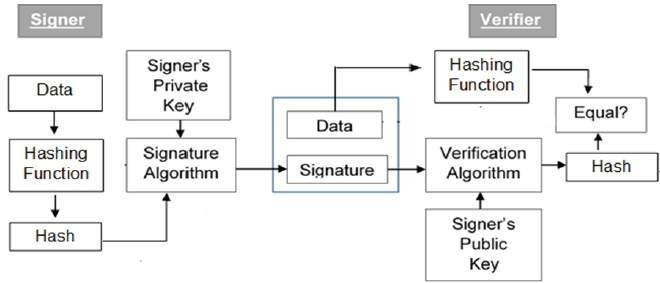
\includegraphics[width=0.8\textwidth]{model_digital_signature.jpg}
\end{center}
\subsection{\textit{Which government agencies are involved to issue the digital signature? What is the validity of digital signature? }}
The government agencies involved in issuing digital signatures can vary depending on the country and its laws and regulations. In some countries, there may be one central agency responsible for issuing digital signatures, while in others, multiple agencies or private companies may be authorized to issue them.\\

For example, in India, the Controller of Certifying Authorities (CCA) is responsible for issuing digital signatures, while in the United States, digital signatures can be obtained from commercial certificate authorities like DigiCert, GlobalSign, and Comodo.\\

The validity of a digital signature can also vary depending on the country and the specific laws and regulations governing digital signatures. In general, a digital signature is considered valid for a certain period of time, after which it may need to be renewed or updated. The validity period can range from a few months to several years, depending on the issuing agency and the type of digital signature.\\

In many countries, digital signatures are governed by laws and regulations that provide legal recognition and validity to electronically signed documents. For example, in the United States, the Electronic Signatures in Global and National Commerce Act (ESIGN) and the Uniform Electronic Transactions Act (UETA) provide a legal framework for the use of digital signatures in electronic transactions.
\end{document}